\chapter{Multipath Analysis}

The overall geometry for analysis of multipath effects on a propagating signal is given in Figure \ref{mp_fig:1}. In this figure, $P_1$ and $P_2$ are the two points we are interested in determining the statistics between. $L_1$ is then the direct path and $L_2 + L_3$ represents the short orbit with a single reflection off the sea surface. The altitude of the two points from the mean sea surface is $h_1$ and $h_2$, respectively and the altitude of the sea surface is $S$. The total downrange distance is $L$ and the distance to the reflection point is $x$.

\begin{figure}[H]
  \begin{center}
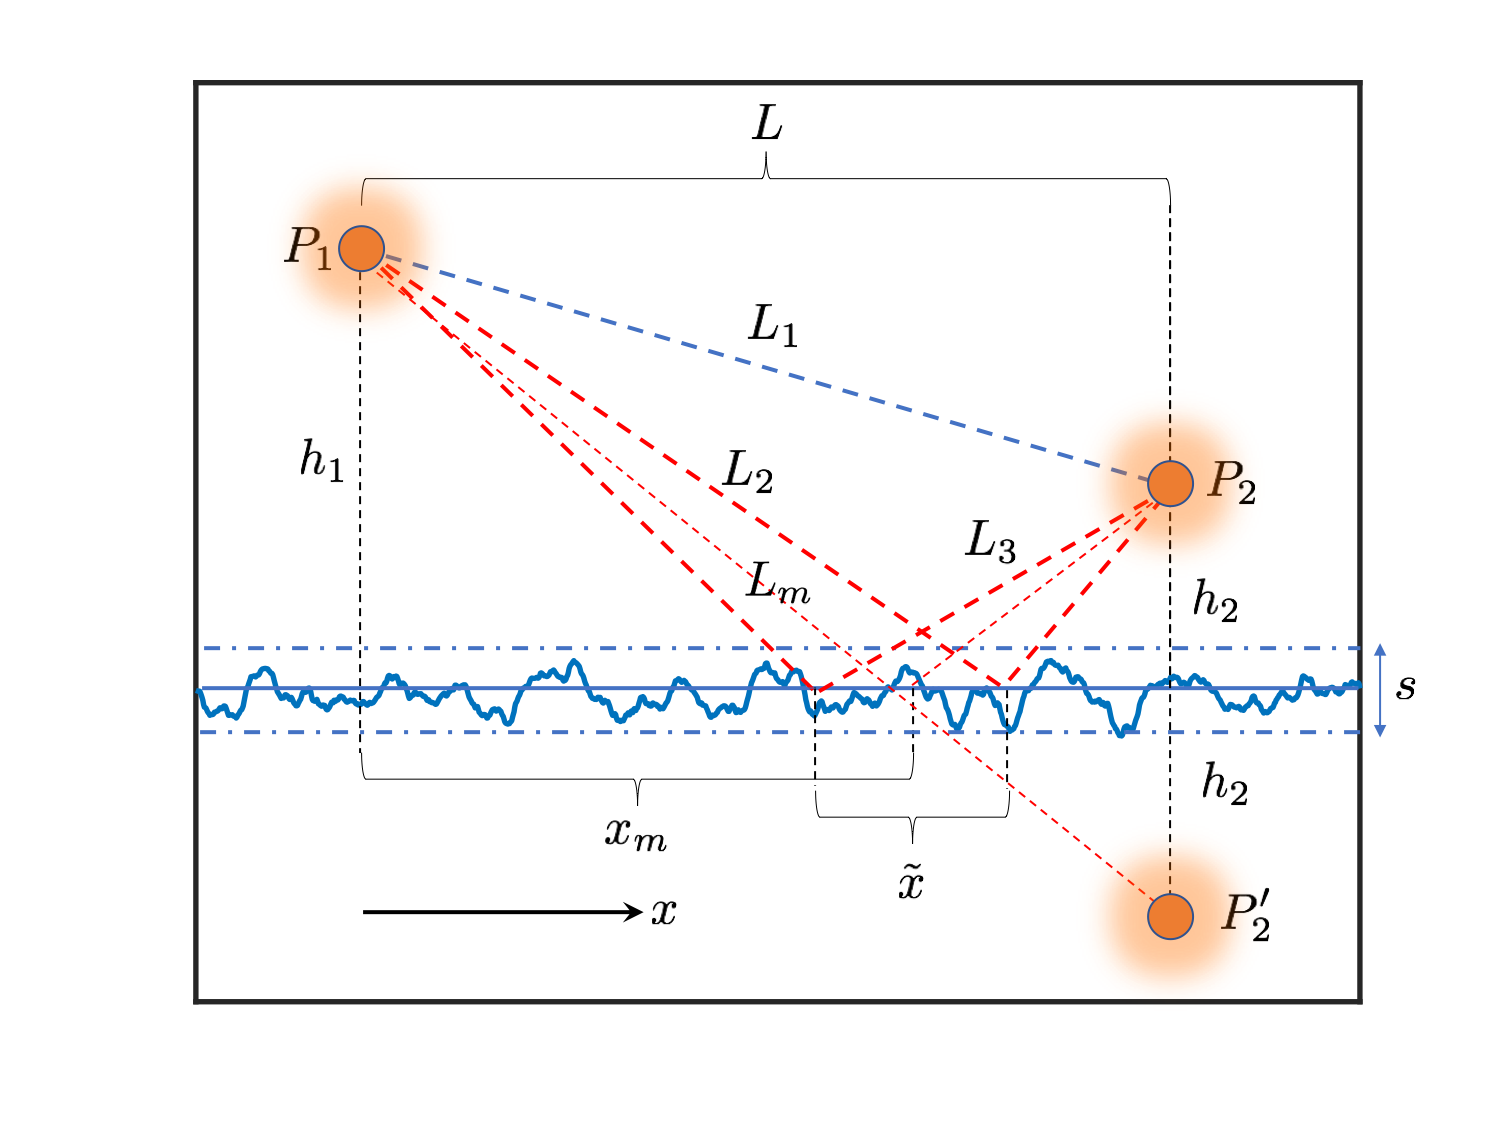
\includegraphics[width=5in]{../media/analysis/multipath_layout.png}
  \end{center}
  \renewcommand{\baselinestretch}{1} \small\normalsize
  \begin{quote}
    \caption[Multipath Geometry]{ Multipath Geometry\label{mp_fig:1}}
  \end{quote}
\end{figure}
\renewcommand{\baselinestretch}{2} \small\normalsize


The path lengths $L_1$, $L_2$ and $L_3$ can be defined through similar triangles about $x$ and can be simplified through a binomial expansion where $s(x)$ specifies the height of the sea surface at the point $x$.
\begin{equation}
\begin{aligned}
L_1 & = \sqrt{L^2 + (h_1-h_2)^2}  \approx L + \frac{(h_1 - h_2)^2}{2L}\\
L_2 &= \sqrt{x^2 + \left( h_1 - s(x)\right)^2}  \approx x + \frac{h_1^2-2h_1s(x)}{2x}\\
L_3 & = \sqrt{\left(L - x\right)^2 + \left( h_2 - s(x)\right)^2}  \approx L-x + \frac{h_2^2 - 2h_2s(x)}{2\left(L-x\right)}\\
\end{aligned}
\label{mp_eq:1}
\end{equation}
\renewcommand{\baselinestretch}{2} \small\normalsize

The path length for the short orbit with a single reflection, $L_{so}$ is then given by
\begin{equation}
\begin{aligned}
L_{so} &= L_2 + L_3 \\
& = x + \frac{h_1^2-2h_1s(x)}{2x} +  L-x + \frac{h_2^2 - 2h_2s(x)}{2\left(L-x\right)} \\
& = L + \frac{1}{2}\left[\frac{h_1^2}{x} + \frac{h_2^2}{L-x} \right] - s(x)\left[ \frac{h_1}{x} + \frac{h_2}{L-x}\right] \\
&= L + L_0 + L_s
\end{aligned}
\label{mp_eq:2}
\end{equation}
\renewcommand{\baselinestretch}{2} \small\normalsize

Here $L$ is the total down range distance (in general, $L \neq L_1$), $L_0$ represents the deterministic component due to reflection from the surface and $L_s$ represents the random component due to reflection from the surface.

We are interested in the region about $x$ where the electromagnetic wave reflects from the surface, so we can perform a Taylor expansion of $L_0$ about its minimum, $x_m$.

\begin{equation}
L_0 \approx L_0(x_m) + \frac{1}{2}\frac{d^2L_0}{dx^2}\bigg|_{x_m}(x-x_m)^2
\label{mp_eq:3}
\end{equation}

\begin{equation}
\frac{dL_0}{dx} = \frac{1}{2}\left[\frac{-h_1^2}{x^2} + \frac{h_2^2}{(L-x)^2} \right]
\label{mp_eq:3}
\end{equation}

\begin{equation}
\frac{d^2L_0}{dx^2} = \frac{h_1^2}{x^3} + \frac{h_2^2}{(L-x)^3} 
\label{mp_eq:3}
\end{equation}

Since $\frac{dL_0}{dx}\big|_{x_m} = 0$, we can solve for $x_m$
\begin{equation}
\begin{gathered}
\frac{-h_1^2}{x_m^2} + \frac{h_2^2}{(L-x_m)^2} = 0\\
\frac{-h_1}{x_m} + \frac{h_2}{L-x_m} = 0\\
\frac{h_1}{x_m} = \frac{h_2}{L-x_m}\\
h_1(L-x_m) = h_2x_m\\
x_m = \frac{h_1L}{h_1+h_2}
\end{gathered}
\label{mp_eq:5}
\end{equation}

We can then expand $L_0$ as
\begin{equation}
L_0 \approx \frac{(h_1+h_2)^2}{2L} + \frac{(h_1+h_2)^4}{h_1h_2L^3}
\label{mp_eq:6}
\end{equation}

We can also express $L_s$ as
\begin{equation}
L_s \approx \frac{2s(x)(h_1 + h_2)}{L}
\label{mp_eq:6a}
\end{equation}

\section{2-Ray Deterministic Approach}
To simplify things, we can let $s(x) \rightarrow 0$, assume $L^3 >> (h_1 - h_2)^4$, and look at the phase difference between the deterministic components, $\varphi$.
\begin{equation}
\begin{aligned}
\varphi &= \frac{2\pi}{\lambda}\left[L_1 - L_{so}\right] = \frac{2\pi}{\lambda}\left[\frac{(h_1-h_2)^2}{2L} - L_0\right]\\
&= \frac{2\pi}{\lambda}\left[\frac{(h_1-h_2)^2}{2L} - \frac{(h_1+h_2)^2}{2L} \right]\\
&= \frac{4\pi h_1h_2}{\lambda L}
\end{aligned}
\label{mp_eq:7}
\end{equation}
\renewcommand{\baselinestretch}{2} \small\normalsize

The derivative of this phase difference with range is $d\varphi/dL$
\begin{equation}
\frac{d\varphi}{dL}=-\frac{4\pi h_1h_2}{\lambda L^2}
\label{mp_eq:8}
\end{equation}

We can convert this derivative from rad/m to rad/sample by multiplying by the spatial sampling distance in range, $\Delta L$.
The derivative of this phase difference with range is $d\varphi/dL$
\begin{equation}
\frac{d\varphi}{dL}=-\frac{4\pi h_1h_2\Delta L}{\lambda L^2}
\label{mp_eq:9}
\end{equation}

Finally, we can insist that this phase shift per sample be smaller than some pre-determined value to provide adequate sampling. It is often convenient to specify this limit in terms of waves and we can enforce the condition that there must be at least $n$ samples per wavelength by 

\begin{equation}
\begin{gathered}
\frac{4\pi h_1h_2\Delta L}{\lambda L^2} \leq \frac{2\pi \lambda}{n}\\
\Delta L \leq \frac{\lambda^2 L^2}{2nh_1h_2}
\end{gathered}
\label{mp_eq:10}
\end{equation}

\section{Multi-Ray Comprehensive Approach}
